\section{Anexos}
\subsection{IVOA Architecture}


El VO's es un framework que ayuda a resolver distintos
problemas que enfrenta la comunidad astronómica a lo largo del mundo.  Uno de
los problemas está relacionado al acceso a los datos, por lo que en IVOA
diseñaron tecnologías y estándares formalmente definidos, que permitan el de
acceso unificado y transparente a distintos servidores con datos astronómicos.

El beneficio que conlleva es considerable, ya que estos
estándares, protocolos, tecnologías y arquitectura, ayudan a la comunidad al
proceso de creación de servicios, portales web, aplicaciones de escritorio,
etc. Todo visto del punto de vista de ingeniería de software.

\subsubsection{Arquitectura VO por Nivel}


IVOA dentro de sus documentos presenta distintos niveles de arquitectura
\cite{ivoa_arch}, con el objetivo de ir aclarando incrementalmente las
funcionalidades (basadas en necesidades) que requiere un VO.

\textbf{Arquitectura Nivel 0} %~\ref{fig:nivel0}\\


La arquitectura más básica que aclara el concepto de VO, se compone por 3
capas:

\begin{enumerate}
    \item Capa de recursos:
          compilado de datos astronómicos provenientes de distintos instrumentos.
    \item Capa de usuarios:
          investigadores que buscan consumir datos.
    \item Capa intermedia:
          es la capa que permite conectar las dos
          capas anteriores de manera transparente para los investigadores.
          Esta interacción se puede llevar a cabo buscando u obteniendo datos.
\end{enumerate}

%\begin{figure*}[h!t]
\begin{figure*}
    \centering
    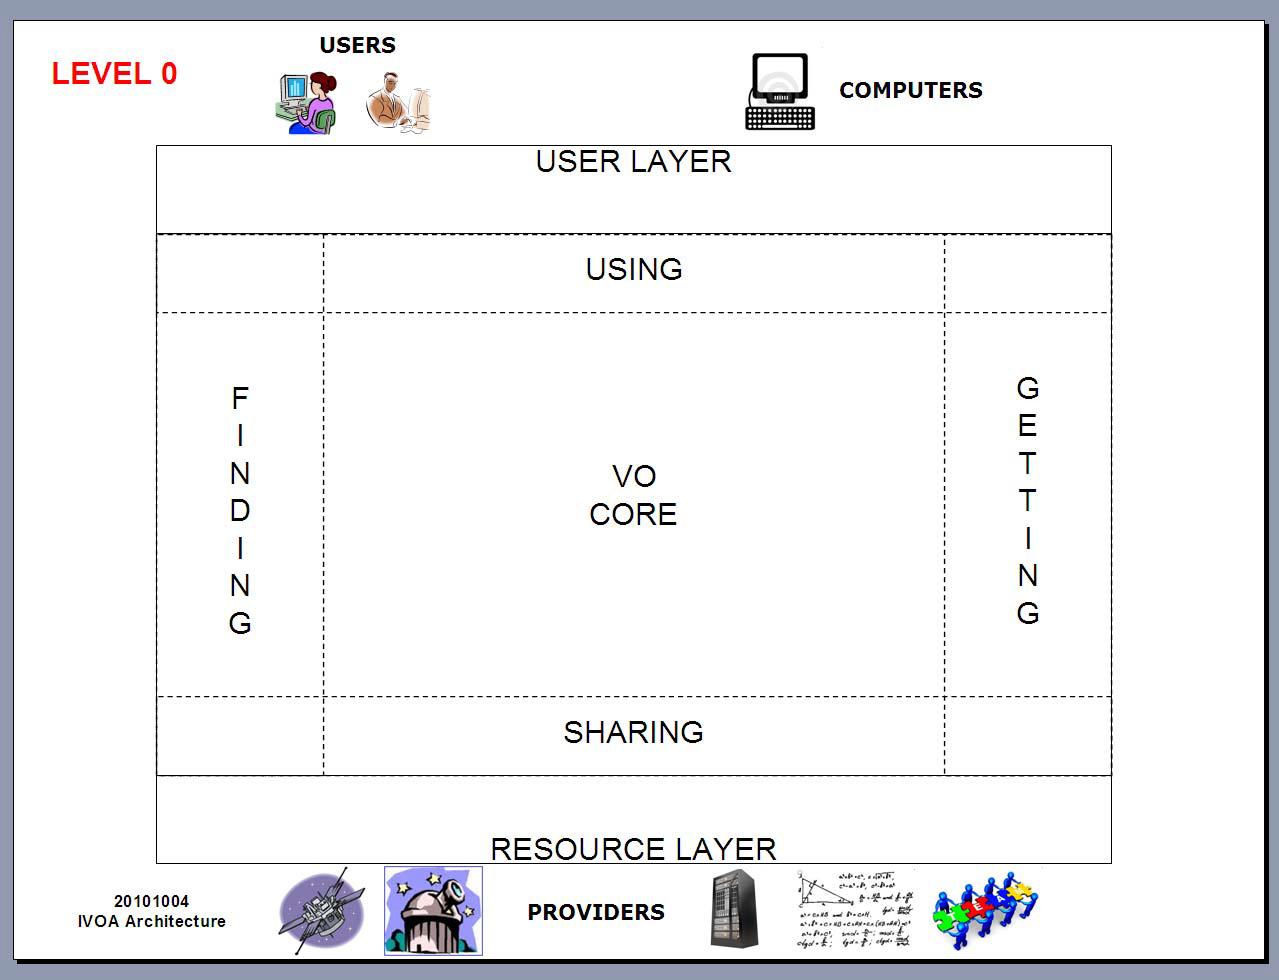
\includegraphics[width=0.7\textwidth]{img/arquitectura_0.png}
    \caption{Arquitectura Nivel 0}
    \label{fig:nivel0}
\end{figure*}

\textbf{Arquitectura Nivel 1}%~\ref{fig:nivel1}


La arquitectura nivel 1 mantiene la misma cantidad de capa pero se especifica:
\begin{enumerate}
    \item Capa de recursos:
          está compuesto de colección de datos y provenientes de distintos
          servidores.
    \item Capa de usuarios:
          un consumidor puede querer acceder a los datos desde un navegador,
          escritorio, o mediante un script.
    \item Capa intermedia:
          crea un framework para compartir los datos, compuesto por VOQL,
          Data Models, Semantics, Formats.
\end{enumerate}

%\begin{figure*}[h!t]
\begin{figure*}
    \centering
    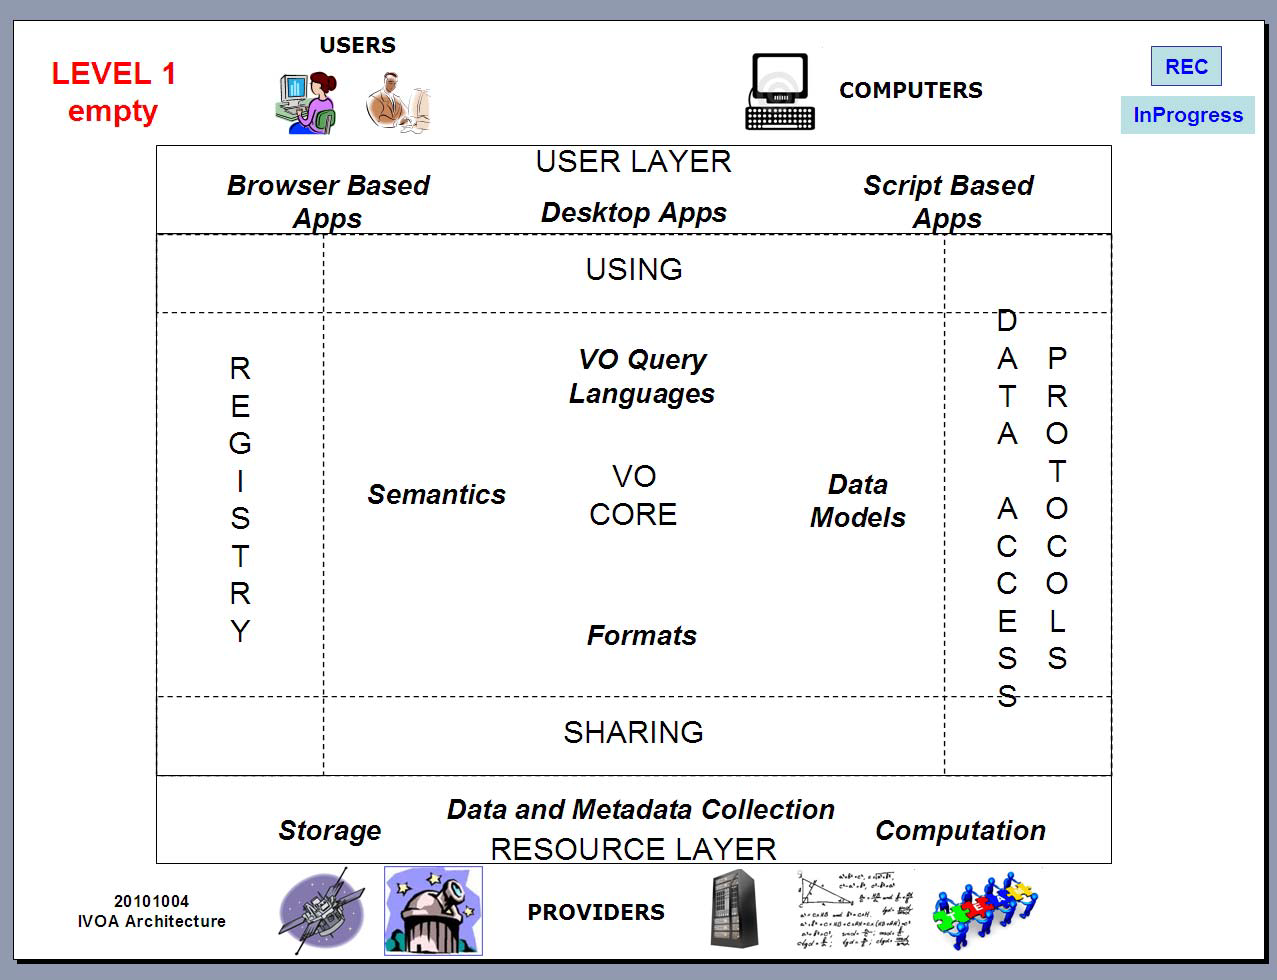
\includegraphics[width=0.7\textwidth]{img/arquitectura_1.png}
    \caption{Arquitectura Nivel 1}
    \label{fig:nivel1}
\end{figure*}

\textbf{Arquitectura Nivel 2}%~\ref{fig:nivel2}


La arquitectura nivel 2 es lo que se entiende por un VO regido por estándares
y protocolos de IVOA.
La idea de esta figura es seccionar cada estándar relacionándolo específicamente
a la capa a la cual pertenece.

%\begin{figure*}[h!t]
\begin{figure*}
    \centering
    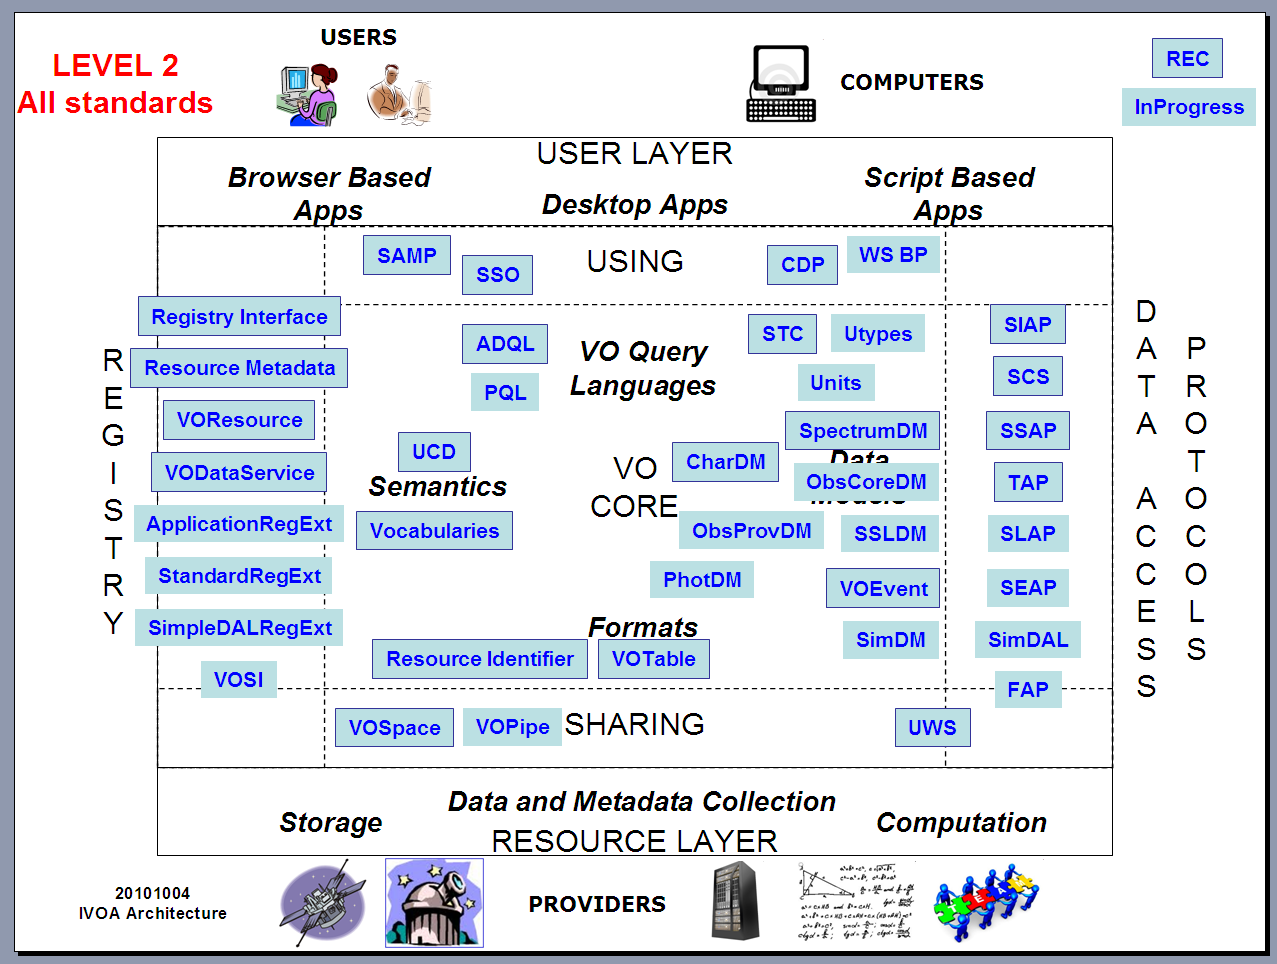
\includegraphics[width=0.7\textwidth]{img/arquitectura_2.png}
    \caption{Arquitectura Nivel 2}
    \label{fig:nivel2}
\end{figure*}


\subsection{Simple Cone Search Protocol}


Este protocolo define una consulta simple para obtener registros desde un
catálogo de fuentes astronómicas. La consulta describe una posición en el cielo
y una distancia angular, definiendo un cono en el cielo. La respuesta retorna
una lista de fuentes astronómicas desde el catálogos cuyas posiciones están
dentro del cono, en formato VOTable.
\url{http://ivoa.net/Documents/latest/ConeSearch.html}

\subsection{Table Access Protocol}


Este protocolo define un servicio general de acceso a datos de tablas,
incluyendo catálogos astronómicos, como también base de datos generales de
tablas. El acceso se provee tanto a la base de datos y a la tabla de metadatos
para la tabla actual. La versión actual del protocolo incluye soporte para
consultas en múltiples lenguajes, incluyendo consultas especificadas en
Astronomical Data Query Language (ADQL) y Parameterised Query Language (PQL).
También incluye soporte para consultas sincrónicas y asíncronas. Este servicio
está ligado netamente al modelo de datos que se usará.
\url{http://www.ivoa.net/documents/TAP/}

\subsection{Simple Image Access Protocol}


Esta especificación define un protocolo para la obtención de datos de imágenes
desde una variedad de repositorios de imágenes astronómicos, a través de una
interfaz uniforme. La interfaz está destinada a ser razonablemente fácil de
implementar por los proveedores de servicios. La query define una región
rectangular en el cielo, la cual es usada para encontrar imágenes candidatas.
El servicio retorna una lista de imágenes en formato VOTable. Por cada imagen
candidata se entrega una URL de referencia, la cual permite acceder a la
imagen. La imagen puede ser retornada en varios formatos gráficos (FITS, JPEG,
etc). \url{http://ivoa.net/Documents/SIA/}

\subsection{Astronomical Data Query Language}


ADQL ha sido desarrollado basándose en SQL92. El estándar describe una conjunto
de gramáticas SQL soportadas(áreas, cajas, círculos, etc). Se han definido
restricciones y extensiones especiales para SQL92 con el objetivo de soportar
operaciones astronómicas genéricas.
\url{http://ivoa.net/Documents/latest/ADQL.html}

\subsection{Semantics}


El grupo de semánticas de IVOA explora las tecnologías en el área de
semánticas, con el objetivo de producir nuevos estándares que ayuden la
interoperabilidad de los sistemas de VO. Este grupo está enfocado en el
significado o la interpretación de las palabras, frases u otras formas de
lenguaje en el contexto de la astronomía. Esto incluye la descripción estándar
de objetos astrofísicos, tipo de datos, conceptos, eventos, o algún otro tipo
de fenómeno en astronomía. Este grupo estudia la relación entre palabras,
símbolos y conceptos, tanto como el significado de esa representación, como por
ejemplo, ontologías. Este grupo cubre el lenguaje natural en astronomía,
incluyendo consultas, traducciones, e internacionalización de interfaces.
\url{http://ivoa.net/twiki/bin/view/IVOA/IvoaSemantics}

\subsection{Simple Spectra Access Protocol}


Este protocolo define una interfaz uniforme para descubrir y acceder
remotamente espectros de una dimensión. Se basa en un modelo de datos más
general, capaz de describir los datos espectrofotométricos, incluyendo series
de tiempo y las distribuciones espectrales de energía (SED), así como 1-D de
espectros. Los conjuntos de datos de candidatos disponibles se describen de
manera uniforme en un documento de formato de VOTable que se devuelve en la
respuesta a la consulta. \url{http://ivoa.net/documents/SSA/}

\subsection{SIMBAD}


Es una base de datos astronómica que provee datos básicos, identificación
cruzada, bibliografía y medidas para objetos astronómicos para objetos fuera
del sistema solar. \url{http://simbad.u-strasbg.fr/simbad/}
